%project-final-report.tex
\documentclass{article}
\usepackage[letterpaper, margin=1.2in]{geometry}
\usepackage{booktabs}
\usepackage{listings}
\usepackage{makecell}
\usepackage{graphicx}
\usepackage{amsmath}
\usepackage{subcaption}
\newcolumntype{L}[1]{>{\raggedright\let\newline\\\arraybackslash\hspace{0pt}}m{#1}}
\newcolumntype{C}[1]{>{\centering\let\newline\\\arraybackslash\hspace{0pt}}m{#1}}
\newcolumntype{R}[1]{>{\raggedleft\let\newline\\\arraybackslash\hspace{0pt}}m{#1}}

\graphicspath{ {images/} }

\begin{document}


\title{An Experiment of Adversarial Exmaples Crafting and Adversarial Training on Various Datasets}
\author{Jian Li \and Mingyue Yang \and David Lie}
\maketitle

\begin{abstract}
In this report, we performed adversarial example crafting and adversarial training on various datasets and evaluated their performance.
\end{abstract}

\section{Introduction}

Goodfellow et\ al. and Papernot et.\ al. introduced several algorithms of crafting \emph{adversarial examples}.
These algorithms include \emph{Fast Gradient Sign Method} (FGSM)\cite{goodfellow2015} and \emph{Jacobian-based Saliency Map Method} (JSMA)\cite{papernot2015}.
We exercised these two adversarial crafting methods on several datasets to find out the relationships between dataset type and performance of the two algorithms.

We constructed several CNNs with TensorFlow\cite{tensorflow} to recognize several datasets.
Then we modified the CNN model to apply adversarial algorithms (implemented by CleverHans\cite{cleverhans}).
We generated adversarial examples with both algorithms and evaluated their success rate for both misclassification and targeted attacks.
Then we retrained the model with adversarial training, and regenerated adversarial examples to evaluate the performance of the adversarial training. Due to limited time frame, we were not able to experiment adversarial training with Saliency Map method.

\section{Datasets}

We crafted adversarial examples using different settings on the datasets shown in Table~\ref{tab:datasetused} below.

\begin{table}[htb]
    \centering
    \begin{tabular}{ | C{0.15\textwidth} | C{0.83\textwidth} | }
    \toprule
    Dataset & Descriptions \\
    \midrule
    GTSRB43 & An image collection consisting of 43 traffic signs captured from real life. Every traffic sign has a serial of images with different resolutions. (32$\times$32 color images) \\ \midrule
    CGTSRB10 & A subset of the original GTSRB\cite{gtsrb} dataset with 10 selected types of traffic signs. (28$\times$28 grey-scale images) \\ \midrule
    CIFAR10 & A collection of real-life objects\cite{cifar10}, containing 60000 samples in 10 classes. (32$\times$32 color images) \\ \midrule
    MNIST & Original MNIST\cite{mnist} dataset with 10 handwritten digits. (28x28 grey-scaled images) \\ \midrule
    FMNIST & Fashion MNIST\cite{fmnist} is a MNIST-like dataset that consists of 10 types of fashion objects such as skirts and shirts. It consists of a training set of 60000 examples and a test set of 10000 examples. (28$\times$28 grey-scale images) \\ \midrule
    MNISTBG & MNIST with background)\cite{mnistbg} is a patched version of MNIST dataset. Each MNIST example is attached with a background image extracted randomly from a set of 20 images downloaded from the Internet. (28$\times$28 grey-scale images) \\ \midrule
    SVHN & Cropped street sign numbers with real-life backgrounds\cite{svhn}. (32x32 color images) \\
    \bottomrule
    \end{tabular}
    \caption{\label{tab:datasetused} List of Datasets Used}
\end{table}

\section{Adversarial Examples Crafting}

We used implementation of the fast gradient sign method and saliency map method from the CleverHans\cite{cleverhans} to craft
adversarial examples for datasets CGTSRB10, CIFAR10, FMNIST, and MNISTBG.
For comparison, we also did the same experiment on original MNIST dataset.


\subsection{Adversarial Examples Crafting with FGSM and JSMA}

\subsubsection{CNN Models}

We trained a convolutional neural network model with TensorFlow\cite{tensorflow} for each dataset.
The legitimate test accuracy is shown in Table \ref{tab:cnnaccuracy}.

\begin{table}
\centering
\begin{tabular}{cc}
    \toprule
    Dataset & Test accuracy \\
    \midrule
    CGTSRB10 & 97\% \\
    CIFAR10 & 68\%  \\
    FMNIST & 92\% \\
    MNISTBG & 92\% \\
    MNIST & 99\% \\
    SVHN & 97\% \\
    \bottomrule
\end{tabular}
\caption{\label{tab:cnnaccuracy} CNN test accuracy with legitimate examples}
\end{table}


\subsubsection{Fast Gradient Sign Method}

For fast gradient sign method, we used 5000 examples from the test set of each dataset (except for CGTSRB10 which has only 3360 test examples)
and generated adversarial examples with \(\epsilon=0.1 \sim 0.6\).
For each example, first a random label different than the example's original label is selected as attack target.
Then the FGSM algorithm is executed to generate an adversarial example.
Finally, the generated adversarial example is fed into the original CNN model to get a prediction,
and the prediction is compared with its original label and the attack target.
If the prediction is identical with attack target then it is a successful targeted attack,
otherwise if the prediction is not the same as the original label, its a successful misclassification.

Figure \ref{fig:fgsm} shows the result of success rate for both misclassification and targeted attacks.

\subsubsection{Saliency Map Method}

For saliency map method, we used the same 5000 examples to generate adversarial examples.
Our plan was to evaluate the performance of different \(\gamma\) parameters.
However, since \(\gamma\) controls the number of iterations, it is not necessary to repeat the execution
on every variation of \(\gamma\).
Therefore we crafted the adversarial examples with \(\gamma=0.15\) while 
recording the iteration count when misclassification and targeted attack succeed with a slightly modified JSMA algorithm.

After the adversarial examples are generated, we calculated the success rate for each planned \(\gamma\) value
with the data recorded during the crafting. Figure \ref{fig:jsma} shows the result of success rate.

\begin{figure}[t!]
    \centering
    \begin{subfigure}[b]{0.49\linewidth}
        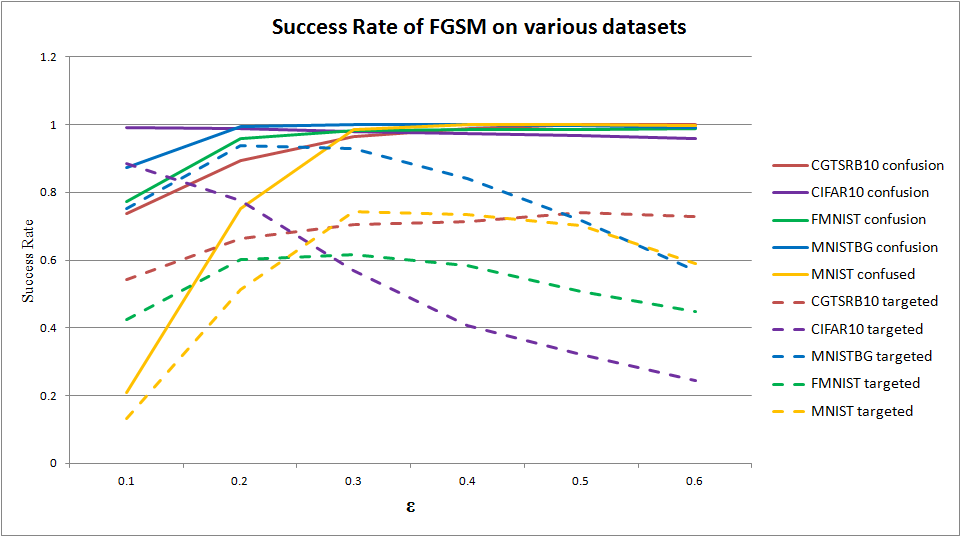
\includegraphics[width=\linewidth]{fgsm}
        \caption{FGSM}
        \label{fig:fgsm}
    \end{subfigure}
    \begin{subfigure}[b]{0.49\linewidth}
        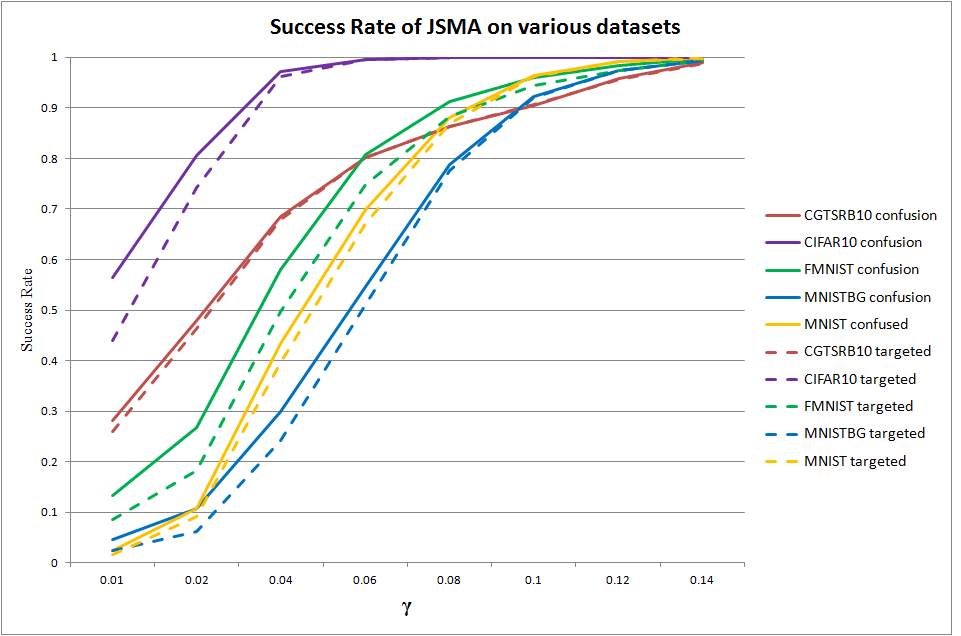
\includegraphics[width=\linewidth]{jsma}
        \caption{JSMA}
        \label{fig:jsma}
    \end{subfigure}
    \caption{Success rate of JSMA and FGSM on various datasets.}
\end{figure}


\subsubsection{Observation}

FGSM can easily confuse CNN model to misclassify an image by altering all the pixels by \(\epsilon\).
For all the datasets, \(\epsilon=0.2\) can easily achieve 80\% success rate on a na\"ive CNN model.
Practically \(\epsilon=0.3\) is easily detectable by human eyes.

However the targeted attacks did not show a good success rate. In most case, targeted success rate starts to fall when \(\epsilon\geq 0.3\).
Intuitively when \(\epsilon\geq 0.3\) the perturbation is enough to confuse human to make wrong classification,
which results in low success rate for targeted attack. However the reason still requires further investigation.

The CNN model for CIFAR10 dataset is easily attacked (misclassification rate $\approx$ 100\% when \(\epsilon=0.1\)),
which is considered the result of its low accuracy (68\%) on legitimate examples.

JSMA gave a good success rate on both misclassification and targeted attacks.
For most datasets, \(\gamma=0.14\) is enough to guarantee 95\% success rate against a na\"ive model.


\subsection{Effect of Number of Epochs on FGSM Whitebox Attack}

To evaluate the effect of number of epoches on FGSM whitebox attack, we did the following experiment based on CNN models listed in Table \ref{tab:cnnaccuracy2}.

\begin{table}
\centering
\begin{tabular}{cc}
    \toprule
    Dataset & Test accuracy \\
    \midrule
    CGTSRB10 & 98\% \\
    FMNIST & 99\% \\
    MNIST & 98\%  \\
    SVHN & 97\% \\
    \bottomrule
\end{tabular}
\caption{\label{tab:cnnaccuracy2} CNN test accuracy with legitimate examples}
\end{table}

FGSM attacks are first performed on models that are cleanly trained with slightly fewer epochs (slightly underfitting).
For comparison, the FGSM attacks are again performed on models that are cleanly trained with slightly more epochs (overfitting).
The accuracy of the 4 models start to show a general trend as $\epsilon$ increases.
When the $\epsilon$ becomes large, models for all the 4 datasets show low accuracy for the FGSM adversarial attack.
It can be observed that all overfitting models are more resistant to attacks with small $\epsilon$ values than their underfitting counterparts.
For attacks with large $\epsilon$ values, however, overfitting models may or may not perform slightly worse on FGSM adversarial samples.

\begin{figure}[h!]
    \centering
    \begin{subfigure}[b]{0.49\textwidth}
        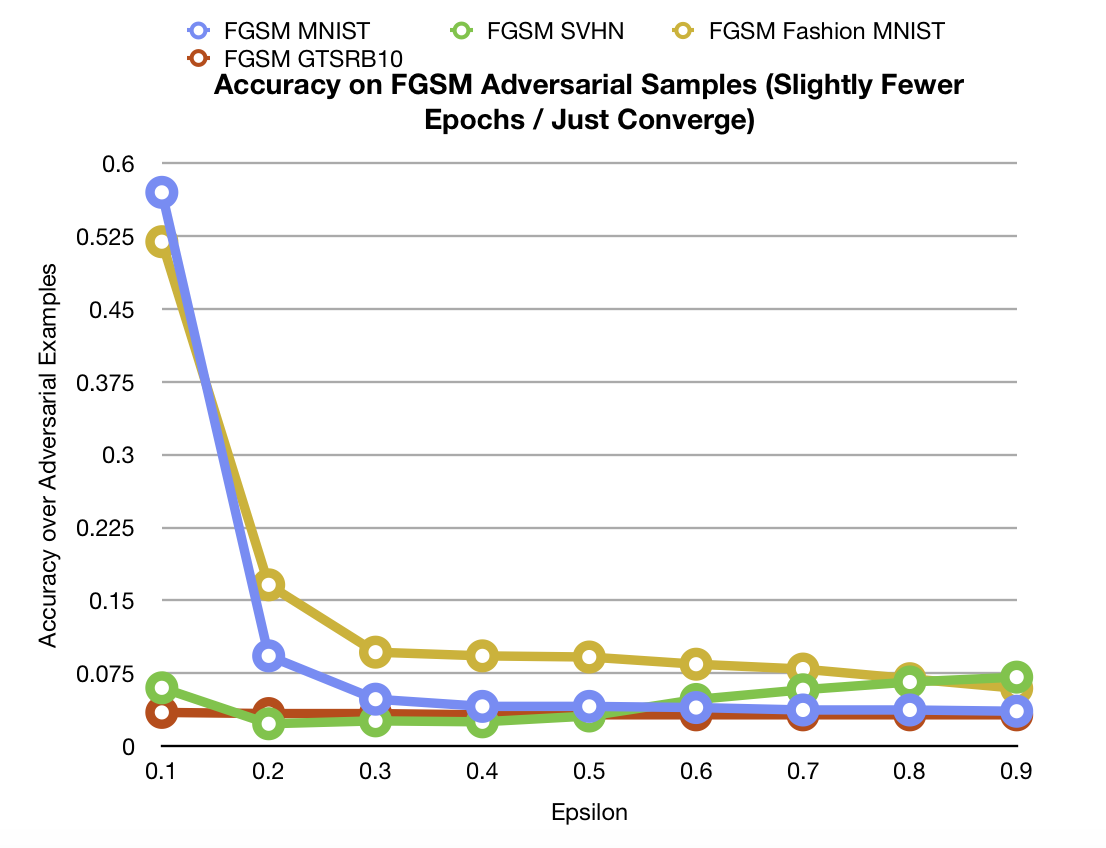
\includegraphics[width=\textwidth]{{image2/2a}.png}
        \caption{Slightly Fewer Epochs}
        \label{fig:fewerfgsm}
    \end{subfigure}
    \begin{subfigure}[b]{0.49\textwidth}
        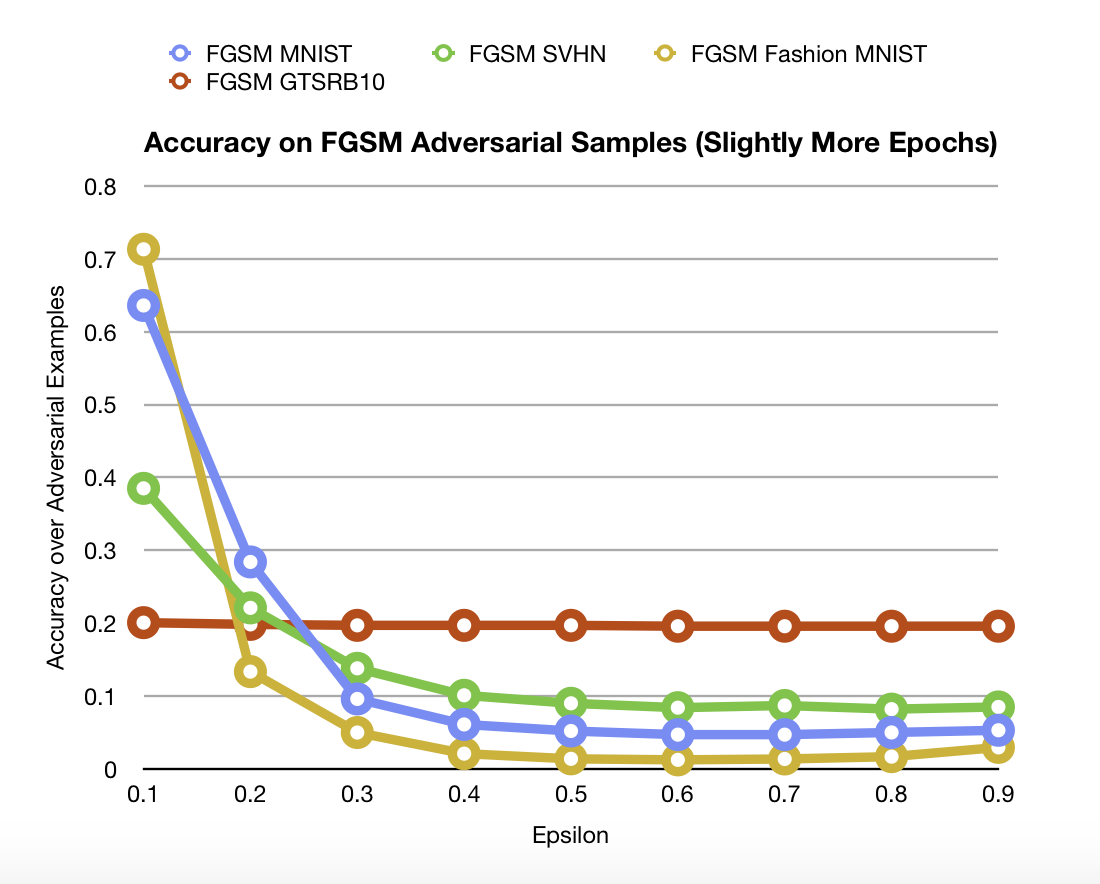
\includegraphics[width=\textwidth]{{image2/2b}.png}
        \caption{Slightly More Epochs}
        \label{fig:morefgsm}
    \end{subfigure}
    \caption{Effect of number of epoches on FGSM whitebox attack}
\end{figure}

\subsection{Effect of Dataset on FGSM Whitebox Attack and Blackbox Attack}

We also evaluated the effect of datasets based on the CNN models in Table \ref{tab:cnnaccuracy2}.
Comparing to models trained with datasets containing noisy backgrounds (GTSRB10 and SVHN), models cleanly trained on dataset with clear background (MNIST and FMNIST) are sustainable to adversarial attacks with a small $\epsilon$ value.
For both the overfitting and underfitting models, MNIST and FMNIST datasets have better accuracy over adversarial samples with small $\epsilon$ values.

\begin{figure}[h!]
    \centering
    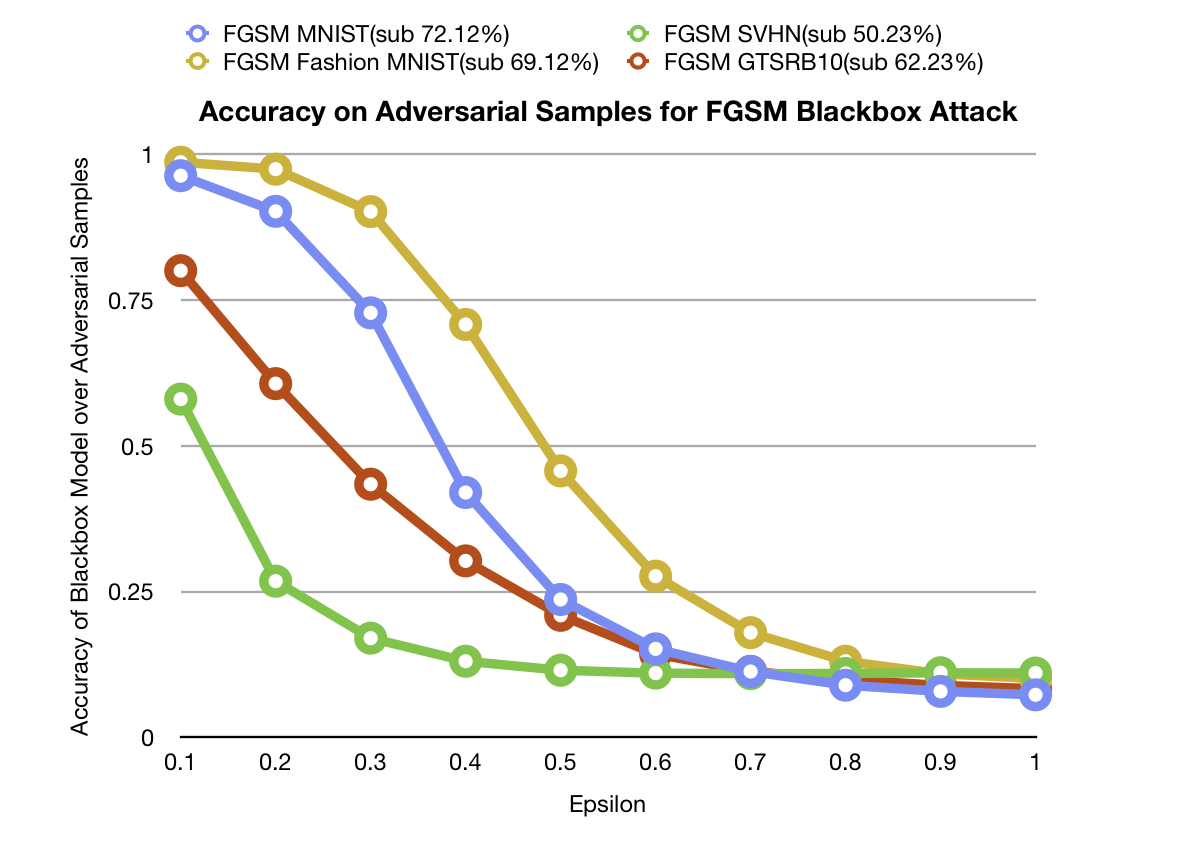
\includegraphics[width=0.49\textwidth]{{image2/3blackbox}.png}
    \label{fig:blackbox}
    \caption{FGSM Blackbox Attack on Different Datasets}
\end{figure}

Then, the FGSM black-box attacks are performed on models trained with all the 4 datasets.
Although we used substitute models with higher accuracy for the MNIST and FMNIST datasets, their accuracy on the adversarial samples are still generally higher than the SVHN and GTSRB10 model.
For MNIST and FMNIST models, the FGSM black-box attacks are hardly successful with a small $\epsilon$ value.
As the $\epsilon$ value increases, the accuracy of all the 4 models decrease in a smooth curvy trend.
The accuracy over adversarial samples converge to around 10\% as the $\epsilon$ value approaches its maximum.
This again demonstrates that models trained with clean-background dataset are more robust under the FGSM attacks with small $\epsilon$ values.


\section{Adversarial Training with FGSM}

Adversarial training is introduced by Goodfellow et\ al.\cite{goodfellow2015}. The fundimental idea is to use adversarial examples as a regularizer:

\[ \tilde{J}(\theta, x, y) = \alpha J(\theta, x, y) + (1 - \alpha)J(\theta, x + \epsilon sign(\nabla_xJ(\theta, x, y))) \]


\subsection{Effect of Adversarial Training}

In the following experiments we used $\alpha=0.5$. First, we train the CNN model with legitimate traning data to get a na\"ive mode.
The test accuracy of these models are listed in Table \ref{tab:cnnaccuracy}.
Then we craft adversarial examples with test data and evaluate the misclassification and targeted success rate.
Next, we do adversarial training three times and regenerate adversarial examples and re-evaluate the success rate after each training session.
We repeated this process with $\alpha=0.1\sim 0.6$ on all the datasets.
Due to space limit, we only picked some of the results (Figure~\ref{fig:trainsucc}), which however could demostrate some interesting facts.

Initially we expected the adversarial training could produce a more robust model that could defense the FGSM attacks. However we found two interesting facts.
Denote the parameter used in adversarial training by $\epsilon$ and the parameter used in following adversarial example crafting by $\tilde{\epsilon}$.

First, a lower $\epsilon$ ($\epsilon = 0.1$) does not provide too much defense against higher $\tilde{\epsilon}$. Especially in the FMNIST dataset, 
even after several adversarial trainings, $\tilde{\epsilon}=0.6$ can still achieve approximately 80\% misclassification rate.

Second, a higher $\epsilon$ does not provide any defense on lower $\tilde{\epsilon}$. When $\epsilon=0.3$, although adversarial examples crafted with $\tilde{\epsilon}=0.3$
can only make less than 10\% success rate, adversarial examples crafted with $\tilde{\epsilon}=0.1$ has higher success rate than $\tilde{\epsilon}=0.3$ and will not decrease
significantly. The similar effect can be seen in $\epsilon=0.5$.

This indicates that adversarial training with various $\tilde{\epsilon}$ may be required in order to train a robust model, however the feasibility is still an open question.

\begin{figure}[h!]
    \centering
    \begin{subfigure}[b]{0.3\textwidth}
        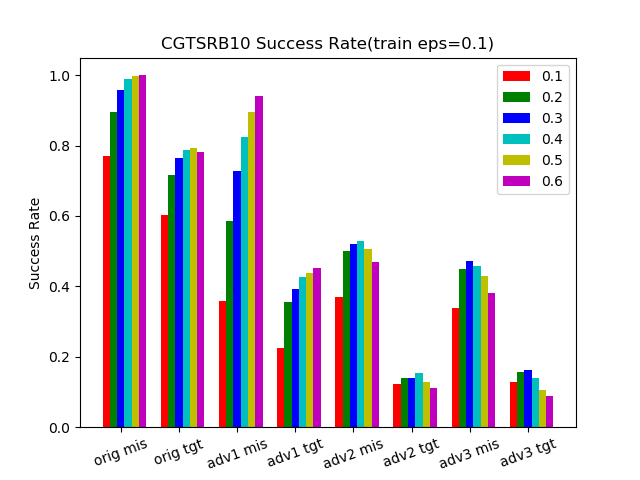
\includegraphics[width=\textwidth]{{eps0.1/sucrate-cgtsrb10-0.1}.png}
        \caption{CGTSRB $\epsilon=0.1$}
    \end{subfigure}
    \begin{subfigure}[b]{0.3\textwidth}
        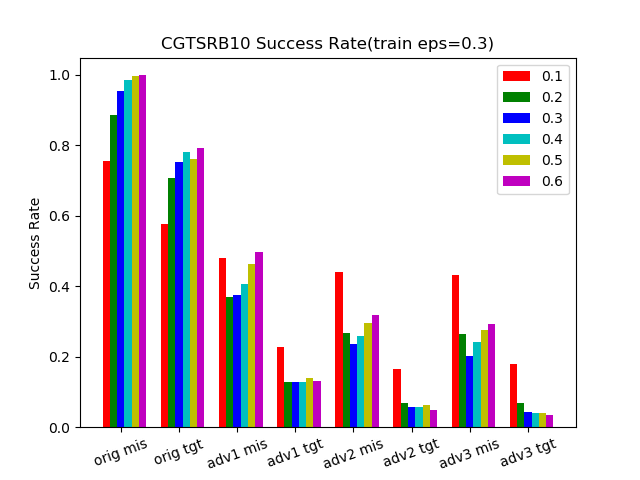
\includegraphics[width=\textwidth]{{eps0.3/sucrate-cgtsrb10-0.3}.png}
        \caption{CGTSRB $\epsilon=0.3$}
    \end{subfigure}
    \begin{subfigure}[b]{0.3\textwidth}
        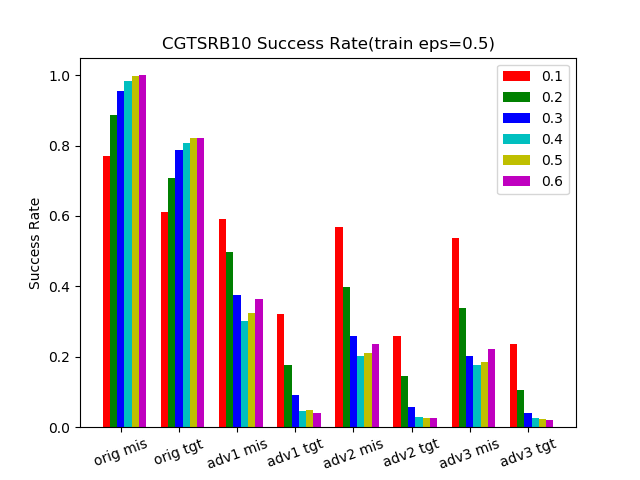
\includegraphics[width=\textwidth]{{eps0.5/sucrate-cgtsrb10-0.5}.png}
        \caption{CGTSRB $\epsilon=0.5$}
    \end{subfigure}

    \begin{subfigure}[b]{0.3\textwidth}
        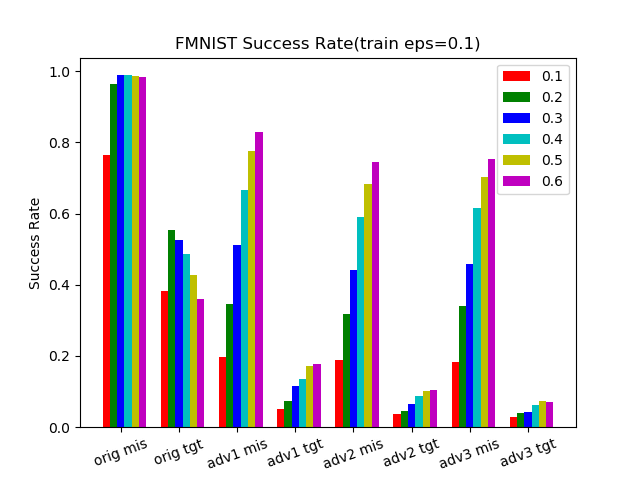
\includegraphics[width=\textwidth]{{eps0.1/sucrate-fmnist-0.1}.png}
        \caption{FMNIST $\epsilon=0.1$}
    \end{subfigure}
    \begin{subfigure}[b]{0.3\textwidth}
        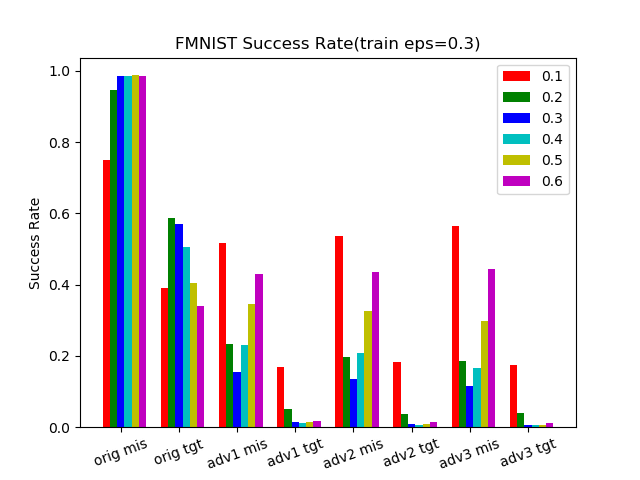
\includegraphics[width=\textwidth]{{eps0.3/sucrate-fmnist-0.3}.png}
        \caption{FMNIST $\epsilon=0.3$}
    \end{subfigure}
    \begin{subfigure}[b]{0.3\textwidth}
        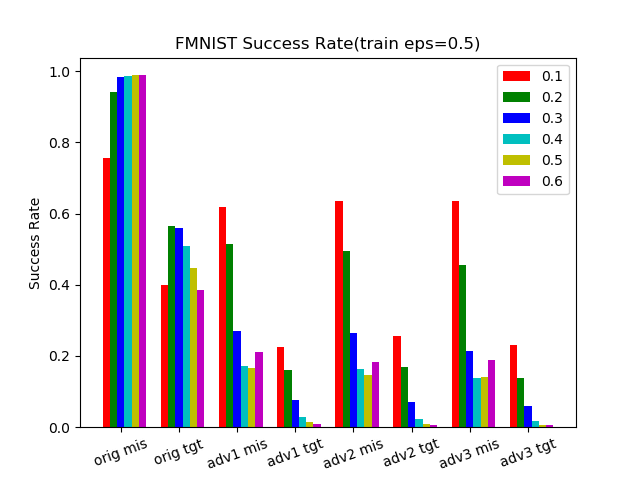
\includegraphics[width=\textwidth]{{eps0.5/sucrate-fmnist-0.5}.png}
        \caption{FMNIST $\epsilon=0.5$}
    \end{subfigure}
    \caption{Success Rate of FGMS with adversarial training. Bars $0.1 \sim 0.6$ are $\tilde{\epsilon}$ used in adversarial example crafting.}
    \label{fig:trainsucc}
\end{figure}


\subsection{Cross-model FGSM Attacks for FGSM Adversarial Training}

Cross-model attack is also performed for models with adversarial training.
For each dataset, the result of cross-model attack is averaged over 5 separate CNN models with $\epsilon$=0.5.
The details of the 5 models used for each dataset is shown in Table \ref{tab:acc5adv} in Appendix.
The FGSM attack first use samples constructed from a CNN model with the same architecture as but different initialization parameter.
Then the adversarial samples are constructed from a DNN model, that has different architecture from the attacked models.
The results are shown in Figure \ref{fig:mnistcross} and Figure \ref{fig:gtsrbcross}.

\begin{figure}[h!]
    \centering
    \begin{subfigure}[b]{0.49\textwidth}
        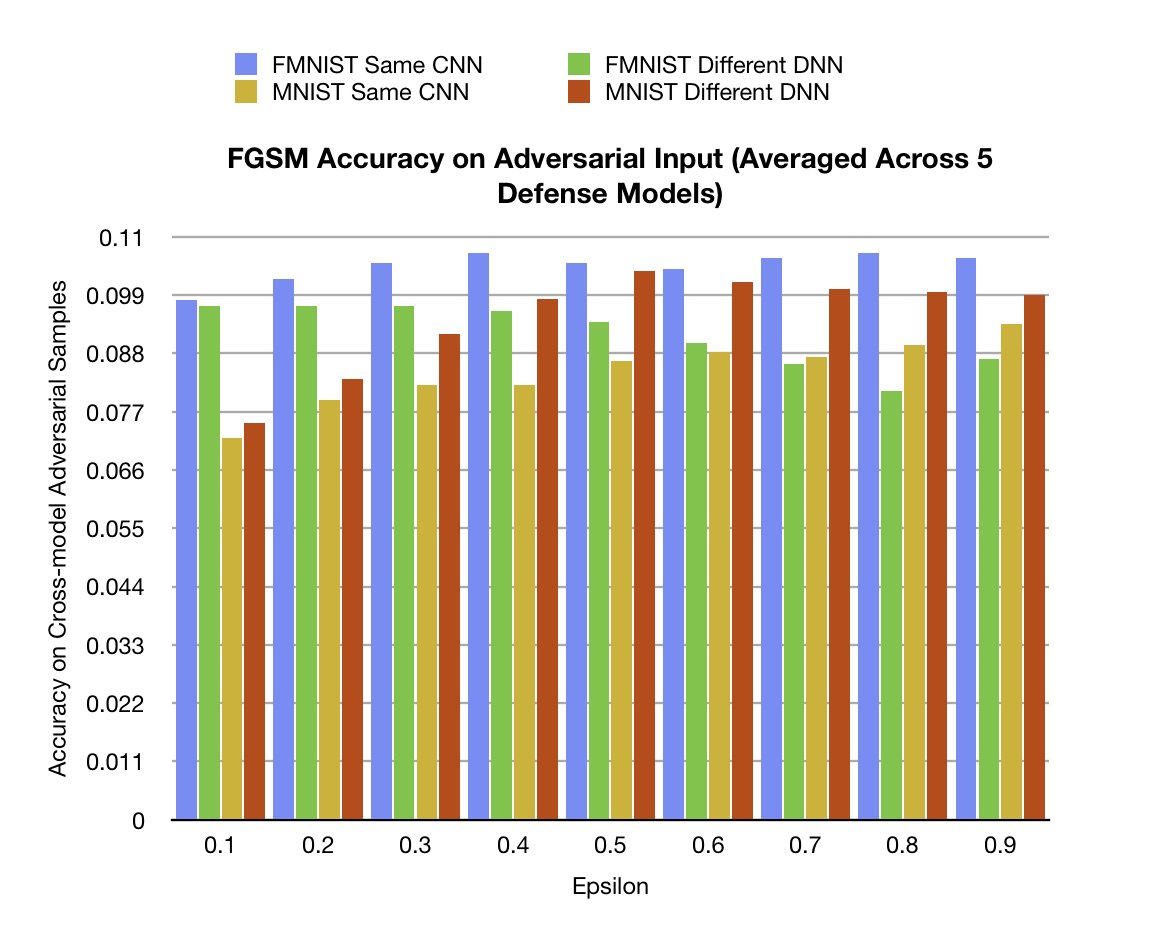
\includegraphics[width=\textwidth]{{image2/5a}.png}
        \caption{MNIST \& FMNIST}
        \label{fig:mnistcross}
    \end{subfigure}
    \begin{subfigure}[b]{0.49\textwidth}
        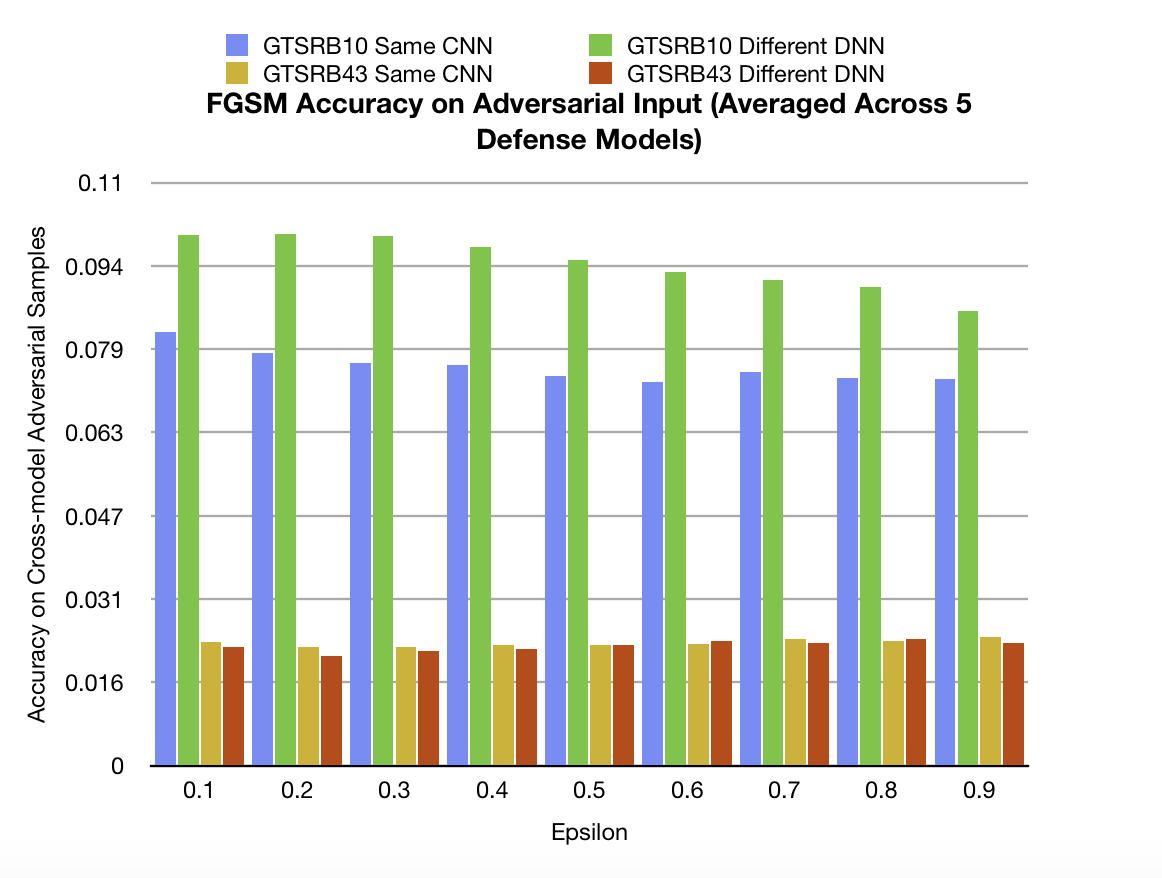
\includegraphics[width=\textwidth]{{image2/5b}.png}
        \caption{GTSRB43 \& GTSRB10}
        \label{fig:gtsrbcross}
    \end{subfigure}
    \caption{Cross-model FGSM Attacks for Adversarial Training}
\end{figure}

Figure \ref{fig:gtsrbcross} shows how GTSRB with different number of classes perform for cross-model attacks.
It can be observe that, the GTSRB10 dataset using only 10 classes from the GTSRB dataset, although obtained a lower adversarial training accuracy, has much higher accuracy than the GTSRB43 dataset which includes all 43 classes.
This result is intuitive: with more classes, it is easier to reach a close class boundary that causes the model to misclassify.

From Figure \ref{fig:mnistcross} and Figure \ref{fig:gtsrbcross}, it can be seen that the different architecture and $\epsilon$ used to construct the adversarial samples do not have much effect on model’s accuracy.
Although there are trends for specific dataset types, no general pattern can be observed. Further exploration may be required to figure out the pattern.
In addition,simple adversarial training, although gives some protection, is still vulnerable to cross-model attacks.


\section{Dataset Distribution}

\begin{figure}[h!]
    \centering
    \begin{subfigure}[b]{0.4\textwidth}
        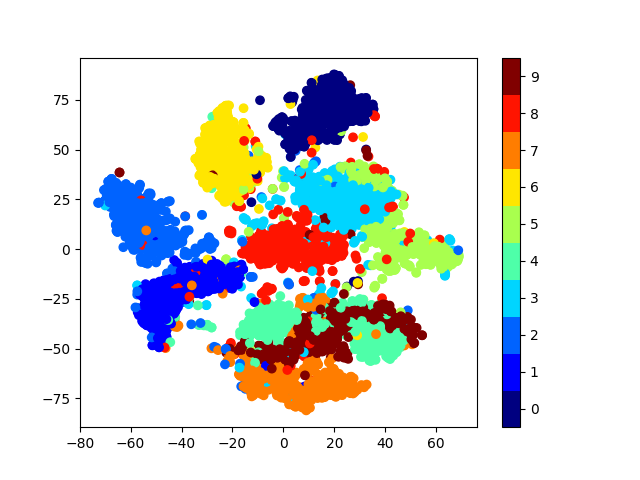
\includegraphics[width=\textwidth]{{image2/6a_mnist}.png}
        \caption{MNIST}
    \end{subfigure}
    \begin{subfigure}[b]{0.4\textwidth}
        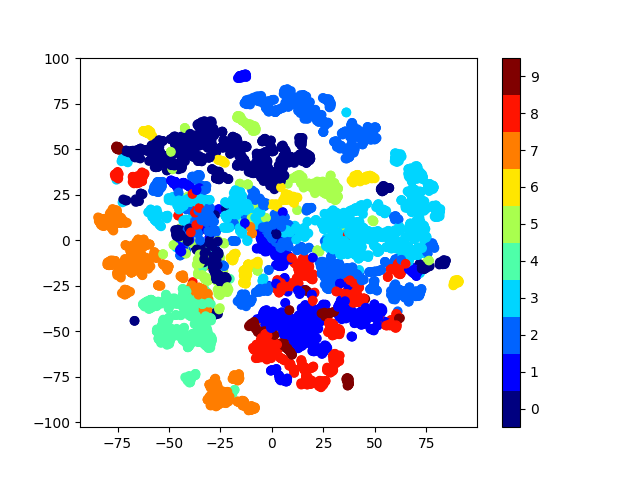
\includegraphics[width=\textwidth]{{image2/6b_gtsrb}.png}
        \caption{GTSRB10}
    \end{subfigure}
    \caption{T-SNE Graphs on MNIST and GTSRB10 Datasets}
    \label{fig:tsneclean}
\end{figure}

To investigate why dataset type can influence accuracy of model over adversarial attacks, the distribution of all datasets is studied.
The T-SNE algorithm is performed on all datasets to obtain a 2D view for the high-dimensional data points.
T-SNE graphs for original clean data are obtained for both the MNIST dataset and the GTSRB10 are shown in Figure \ref{fig:tsneclean}.
From the graphs, it can be observed that the MNIST dataset have more easily distinguishable clusters with clear boundaries, while the clusters for the GTSRB10 dataset are more scattered.
This is due to the fact that the MNIST dataset are simpler images with clear background, while the GTSRB10 dataset has a noisy background.
This result also holds for other datasets that have clear/noisy background.
The complexity and lack of clear boundary may contribute to the fact that of datasets with noisy backgrounds are more susceptible to attacks with small $\epsilon$ values.

\begin{figure}[h!]
    \centering
    \begin{subfigure}[b]{0.3\textwidth}
        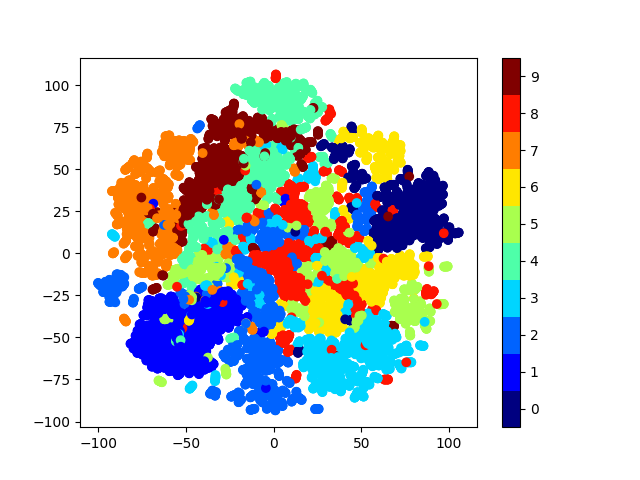
\includegraphics[width=\textwidth]{{image2/7a_mnist_by_class}.png}
        \caption{Clean \& Adversarial Samples Classifed by Original Class}
        \label{fig:tsne7a}
    \end{subfigure}
    \begin{subfigure}[b]{0.3\textwidth}
        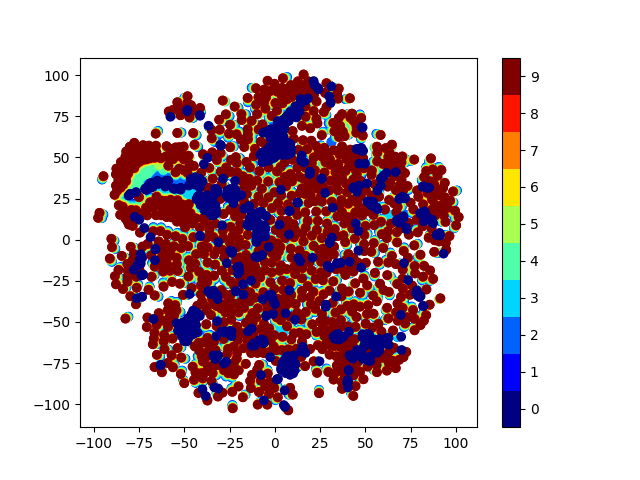
\includegraphics[width=\textwidth]{{image2/7b_mnist_by_epsilon}.png}
        \caption{Clean \& Adversarial Samples from All Classes, Classified by $\epsilon$}
        \label{fig:tsne7b}
    \end{subfigure}
    \begin{subfigure}[b]{0.3\textwidth}
        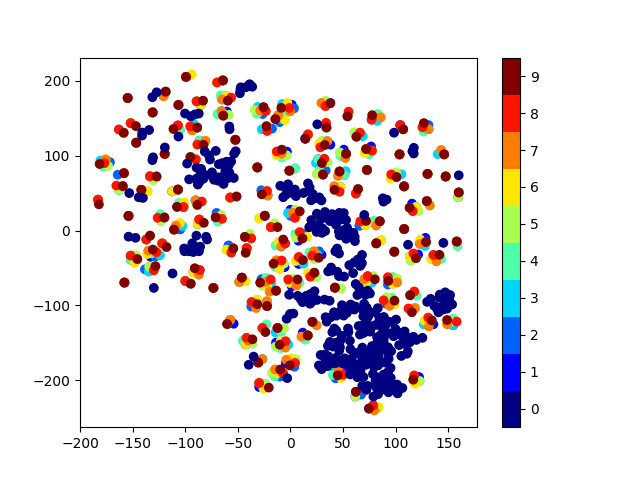
\includegraphics[width=\textwidth]{{image2/7c_mnist_specific_class}.png}
        \caption{Clean \& Adversarial Samples from Single Class, Classified by $\epsilon$}
        \label{fig:tsne7c}
    \end{subfigure}
    \caption{T-SNE Graphs of Adversarial and Clean Samples from MNIST}
\end{figure}

To show how the adversarial samples and original clean samples are different, the T-SNE algorithm is again performed on both original samples and FGSM adversarial samples of the MNIST dataset.
For data labelled by their original class, data points in same original class form distinguishable clusters.
For data labelled using $\epsilon$ values from 0~0.9, adversarial data points all scatter over the 2D space, while original clean data form many small clusters in the 2D space.
The boundary between the adversarial and clean data points is not clear.
This shows that although the FGSM adversarial samples are able to fool the attacked models, from the T-SNE perspective, FGSM adversarial samples can still be distinguished by their original class, and the common patterns in adversarial samples are not obvious.

For further investigation, a specific MNIST class is picked, and T-SNE is performed on both FGSM adversarial samples and original clean samples in this specific class.
In this specific class, original clean data from a distinguishable cluster, while the adversarial samples scatter over the space and there is no boundary between samples with different $\epsilon$ values.
This indicates that it is possible to separate adversarial samples and original clean data given the original class.
This suggests a possibility to build a separately trained machine learning classifier that differentiates adversarial samples from clean samples.


\section{Conclusion}

We experimented adversarial example crafting on various datasets and demostrated the success rate of fast gradient sign method and saliency map method on each dataset.
We also experimented FGSM adversarial training and found that various $\epsilon$ values may be required to obtain a robust model with adversarial training.

For cleanly trained models, we found that slightly overfitting models and simple datasets with clean backgrounds are better at sustaining FGSM attacks.
Investigation shows the class boundaries are more clear for simplers datasets.
In addition, we observe that adversarial training on simpler datasets have better effects.
Adversarial training, although gives some defenses, is still susceptible to cross-model attacks.
Increasing the number of classes in dataset also makes cross-model attacks easier.


\begin{thebibliography}{9}
\raggedright
\bibitem{goodfellow2015}
    Goodfellow, Ian J et\ al.,
    \emph{Explaining and Harnessing Adversarial Examples},  
    arXiv:1412.6572v3,
    3/2015

\bibitem{papernot2015}
    Nicolas Papernot et.\ al.,
   \emph{The Limitations of Deep Learning in Adversarial Settings},
    arXiv 1511.07528v1,
    11/2015

\bibitem{blackbox2017}
    Nicolas Papernot et.\ al.,
    \emph{Practical Black-Box Attacks against Machine Learning}.
    ASIA CCS '17,
    2017.

\bibitem{cifar10}
    \emph{The CIFAR-10 dataset},
    https://www.cs.toronto.edu/~kriz/cifar.html

\bibitem{gtsrb}
    \emph{German Traffic Sign Recognition Benchmark}.
    http://benchmark.ini.rub.de/?section=gtsrb\&subsection=dataset

\bibitem{fmnist}
    \emph{Fashion MNIST},
    https://github.com/zalandoresearch/fashion-mnist

\bibitem{mnistbg}
    \emph{MNIST with Background},
    http://www.iro.umontreal.ca/~lisa/twiki/bin/view.cgi/Public/MnistVariations

\bibitem{mnist}
    \emph{MNIST},
    http://yann.lecun.com/exdb/mnist/

\bibitem{svhn}
    \emph{The Street View House Numbers(SVHN) Dataset},
    http://ufldl.stanford.edu/housenumbers/

\bibitem{cleverhans}
    \emph{CleverHans},
    https://github.com/tensorflow/cleverhans

\bibitem{tensorflow}
    \emph{TensorFlow},
    http://tensorflow.org/

\end{thebibliography}



\section{Appendix}
\begin{table} [htbp]
\centering
\begin{tabular}{ccc}
    \toprule
    Model After Adversarial Training \(\epsilon=0.5\) & Accuracy on Legitimate Examples & Accuracy on Adversarial Examples \\
    \midrule
    FMNIST 1 & 0.991 & 0.991 \\
    FMNIST 2 & 0.992 & 0.992 \\
    FMNIST 3 & 0.991 & 0.990 \\
    FMNIST 4 & 0.991 & 0.990 \\
    FMNIST 5 & 0.992 & 0.992 \\
    MNIST 1 & 0.985 & 0.981 \\
    MNIST 2 & 0.982 & 0.978 \\
    MNIST 3 & 0.982 & 0.980 \\
    MNIST 4 & 0.989 & 0.983 \\
    MNIST 5 & 0.982 & 0.977 \\
    GTSRB10 1 & 0.999 & 0.998 \\
    GTSRB10 2 & 0.998 & 0.995 \\
    GTSRB10 3 & 0.999 & 0.997 \\
    GTSRB10 4 & 0.999 & 0.998 \\
    GTSRB10 5 & 0.999 & 0.998 \\

    GTSRB43 1 & 0.980 & 0.942 \\
    GTSRB43 2 & 0.976 & 0.960 \\
    GTSRB43 3 & 0.974 & 0.939 \\
    GTSRB43 4 & 0.979 & 0.968 \\
    GTSRB43 5 & 0.978 & 0.944 \\
    \bottomrule
\end{tabular}
\caption{\label{tab:acc5adv} Accuracy of Model After Adversarial Training \(\epsilon=0.5\) }
\end{table}




\end{document}
